% TikZ Figures for the Paper

\usepackage{tikz}
\usetikzlibrary{shapes, arrows, positioning, fit, calc, trees}
\usetikzlibrary{arrows.meta}
\usetikzlibrary{backgrounds}

% Figure 1: System Architecture
\begin{figure}[htbp]
\centering
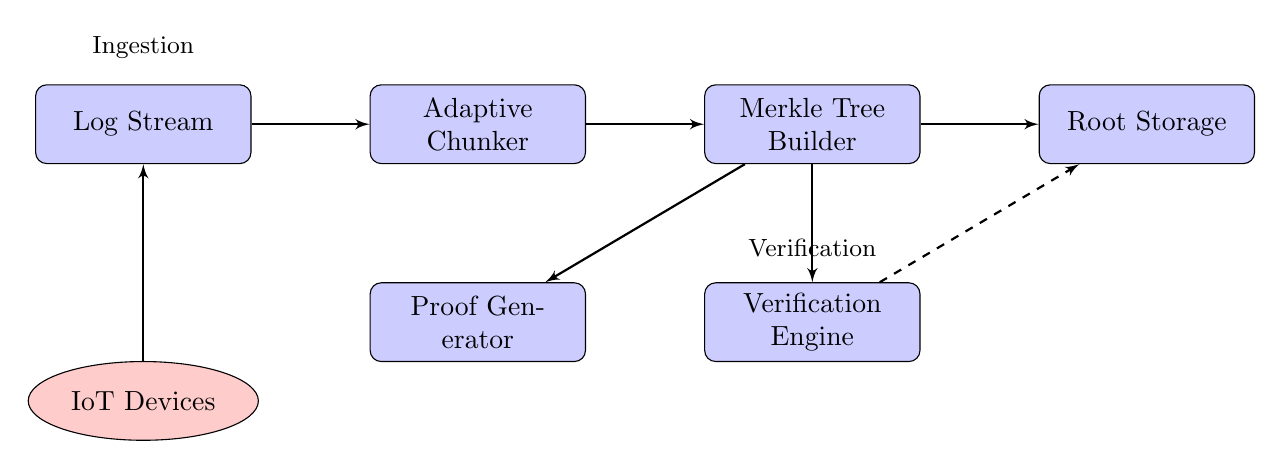
\begin{tikzpicture}[
    node distance=1.5cm,
    block/.style={rectangle, draw, fill=blue!20, text width=2.5cm, text centered, rounded corners, minimum height=1cm},
    line/.style={draw, -latex', thick},
    cloud/.style={draw, ellipse, fill=red!20, node distance=2.5cm, minimum height=1cm}
]

% Nodes
\node [block] (logs) {Log Stream};
\node [block, right=of logs] (chunker) {Adaptive Chunker};
\node [block, right=of chunker] (merkle) {Merkle Tree Builder};
\node [block, right=of merkle] (root) {Root Storage};
\node [block, below=of merkle] (verify) {Verification Engine};
\node [block, left=of verify] (proof) {Proof Generator};
\node [cloud, below=of logs] (iot) {IoT Devices};

% Lines
\path [line] (logs) -- (chunker);
\path [line] (chunker) -- (merkle);
\path [line] (merkle) -- (root);
\path [line] (merkle) -- (verify);
\path [line] (merkle) -- (proof);
\path [line] (iot) -- (logs);
\path [line, dashed] (verify) -- (root);

% Labels
\node [above=0.2cm of logs] {\small Ingestion};
\node [above=0.2cm of verify] {\small Verification};

\end{tikzpicture}
\caption{System Architecture for Lightweight Log Integrity Verification}
\label{fig:architecture}
\end{figure}

% Figure 2: Merkle Tree Construction
\begin{figure}[htbp]
\centering
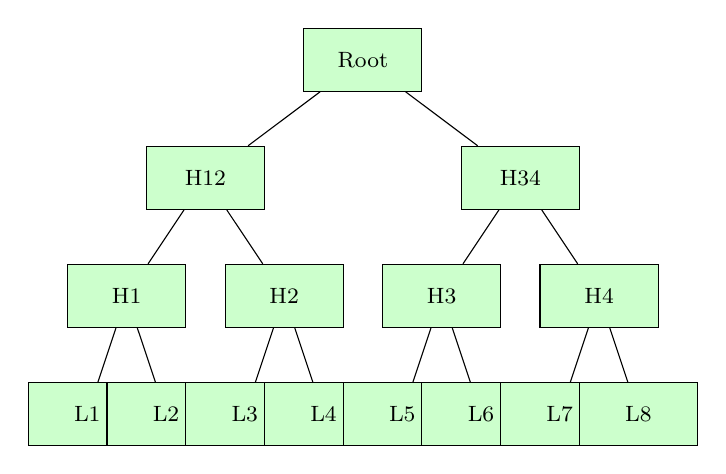
\begin{tikzpicture}[
    level 1/.style={sibling distance=4cm},
    level 2/.style={sibling distance=2cm},
    level 3/.style={sibling distance=1cm},
    every node/.style={rectangle, draw, fill=green!20, minimum width=1.5cm, minimum height=0.8cm, font=\footnotesize}
]

\node {Root}
    child {node {H12}
        child {node {H1}
            child {node {L1}}
            child {node {L2}}
        }
        child {node {H2}
            child {node {L3}}
            child {node {L4}}
        }
    }
    child {node {H34}
        child {node {H3}
            child {node {L5}}
            child {node {L6}}
        }
        child {node {H4}
            child {node {L7}}
            child {node {L8}}
        }
    };

\end{tikzpicture}
\caption{Merkle Tree Construction for Log Integrity}
\label{fig:merkle}
\end{figure}

% Figure 3: Adaptive Chunking Algorithm
\begin{figure}[htbp]
\centering
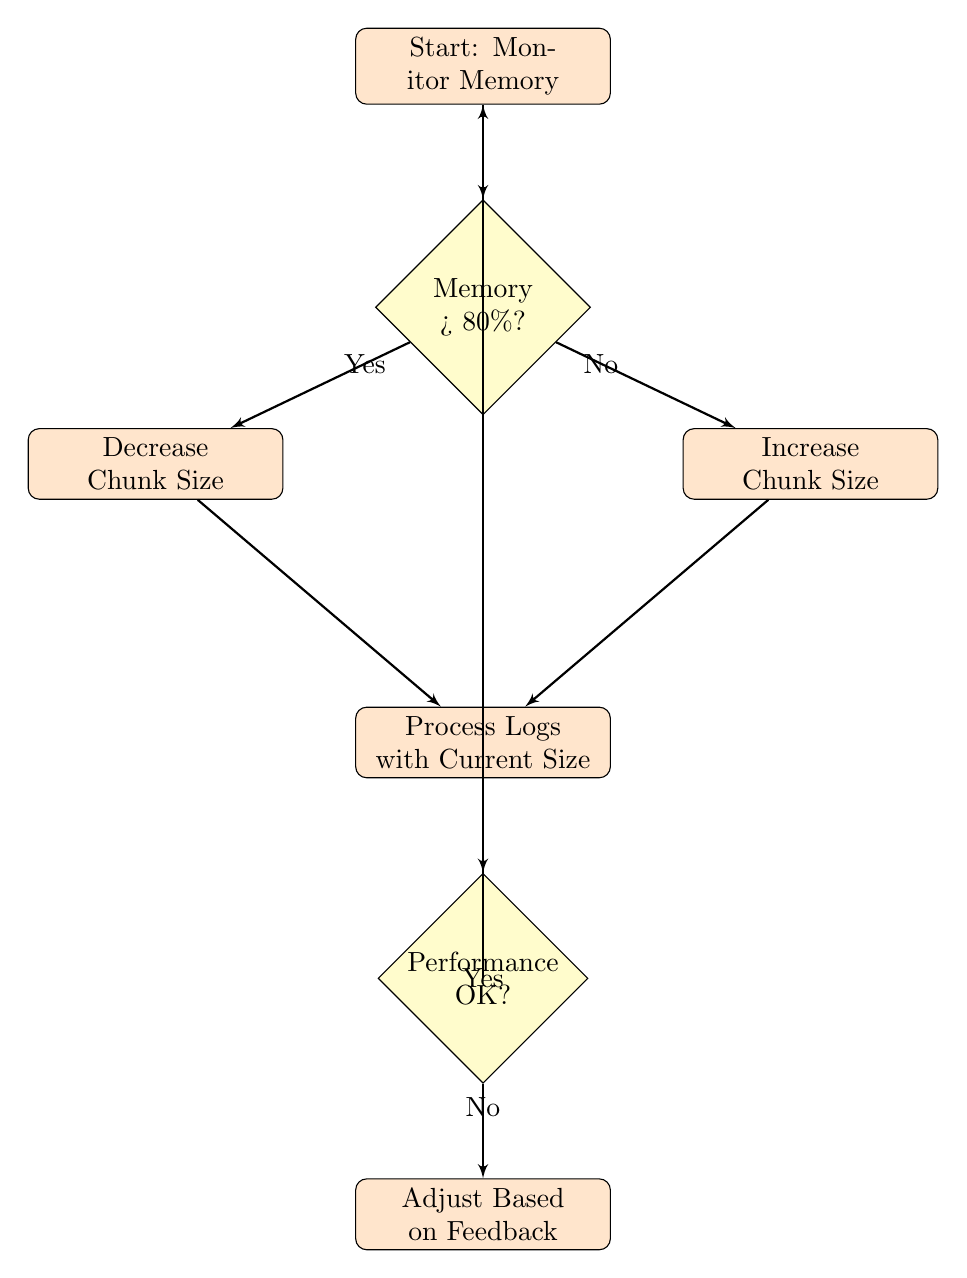
\begin{tikzpicture}[
    node distance=1.2cm,
    block/.style={rectangle, draw, fill=orange!20, text width=3cm, text centered, rounded corners, minimum height=0.8cm},
    decision/.style={diamond, draw, fill=yellow!20, text width=2cm, text centered, inner sep=0pt},
    line/.style={draw, -latex', thick}
]

\node [block] (start) {Start: Monitor Memory};
\node [decision, below=of start] (check) {Memory > 80\%?};
\node [block, below left=of check, xshift=-1cm] (decrease) {Decrease Chunk Size};
\node [block, below right=of check, xshift=1cm] (increase) {Increase Chunk Size};
\node [block, below=of check, yshift=-2.5cm] (process) {Process Logs with Current Size};
\node [decision, below=of process] (feedback) {Performance OK?};
\node [block, below=of feedback] (adjust) {Adjust Based on Feedback};

\path [line] (start) -- (check);
\path [line] (check) -- node [near start] {Yes} (decrease);
\path [line] (check) -- node [near start] {No} (increase);
\path [line] (decrease) -- (process);
\path [line] (increase) -- (process);
\path [line] (process) -- (feedback);
\path [line] (feedback) -- node [near start] {No} (adjust);
\path [line] (feedback) -| node [near start] {Yes} (start);

\end{tikzpicture}
\caption{Adaptive Chunking Algorithm Flow}
\label{fig:chunking}
\end{figure}

% Figure 4: Verification Process
\begin{figure}[htbp]
\centering
\begin{tikzpicture}[
    node distance=1.5cm,
    block/.style={rectangle, draw, fill=purple!20, text width=2.5cm, text centered, rounded corners, minimum height=0.8cm},
    line/.style={draw, -latex', thick}
]

\node [block] (request) {Verification Request};
\node [block, right=of request] (proof) {Generate Merkle Proof};
\node [block, right=of proof] (compute) {Compute Root from Proof};
\node [decision, below=of compute] (compare) {Roots Match?};
\node [block, right=of compare, xshift=1cm] (valid) {Valid: Integrity Verified};
\node [block, left=of compare, xshift=-1cm] (invalid) {Invalid: Tampering Detected};

\path [line] (request) -- (proof);
\path [line] (proof) -- (compute);
\path [line] (compute) -- (compare);
\path [line] (compare) -- node [near start] {Yes} (valid);
\path [line] (compare) -- node [near start] {No} (invalid);

\end{tikzpicture}
\caption{Log Entry Verification Process}
\label{fig:verification}
\end{figure}

% Figure 5: Performance Comparison
\begin{figure}[htbp]
\centering
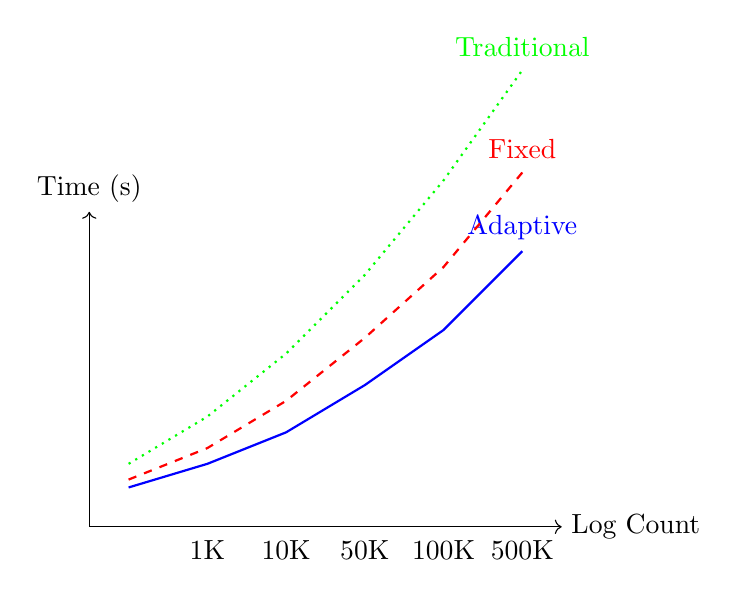
\begin{tikzpicture}
\draw[->] (0,0) -- (6,0) node[right] {Log Count};
\draw[->] (0,0) -- (0,4) node[above] {Time (s)};

% Adaptive chunking
\draw[blue, thick] (0.5,0.5) -- (1.5,0.8) -- (2.5,1.2) -- (3.5,1.8) -- (4.5,2.5) -- (5.5,3.5);
\node[blue] at (5.5,3.8) {Adaptive};

% Fixed chunking
\draw[red, thick, dashed] (0.5,0.6) -- (1.5,1.0) -- (2.5,1.6) -- (3.5,2.4) -- (4.5,3.3) -- (5.5,4.5);
\node[red] at (5.5,4.8) {Fixed};

% Traditional
\draw[green, thick, dotted] (0.5,0.8) -- (1.5,1.4) -- (2.5,2.2) -- (3.5,3.2) -- (4.5,4.4) -- (5.5,5.8);
\node[green] at (5.5,6.1) {Traditional};

% X-axis labels
\node at (1.5,-0.3) {1K};
\node at (2.5,-0.3) {10K};
\node at (3.5,-0.3) {50K};
\node at (4.5,-0.3) {100K};
\node at (5.5,-0.3) {500K};

\end{tikzpicture}
\caption{Ingestion Time Comparison (Lower is Better)}
\label{fig:performance}
\end{figure}

% Figure 6: Security Properties
\begin{figure}[htbp]
\centering
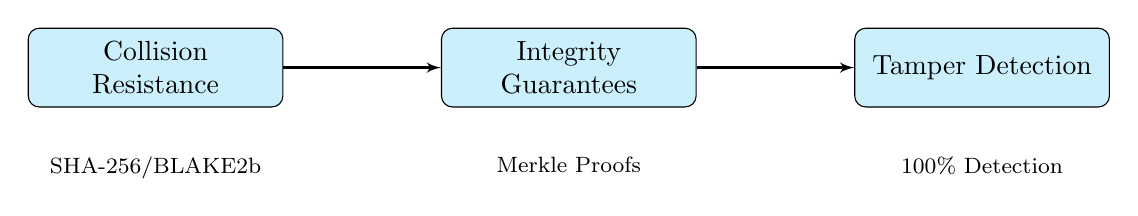
\begin{tikzpicture}[
    node distance=2cm,
    block/.style={rectangle, draw, fill=cyan!20, text width=3cm, text centered, rounded corners, minimum height=1cm},
    line/.style={draw, -latex', thick}
]

\node [block] (collision) {Collision Resistance};
\node [block, right=of collision] (integrity) {Integrity Guarantees};
\node [block, right=of integrity] (detection) {Tamper Detection};

\node [below=0.5cm of collision, text width=3cm, text centered, font=\footnotesize] {SHA-256/BLAKE2b};
\node [below=0.5cm of integrity, text width=3cm, text centered, font=\footnotesize] {Merkle Proofs};
\node [below=0.5cm of detection, text width=3cm, text centered, font=\footnotesize] {100\% Detection};

\path [line] (collision) -- (integrity);
\path [line] (integrity) -- (detection);

\end{tikzpicture}
\caption{Security Properties of the Proposed System}
\label{fig:security}
\end{figure}
